%%%%%%%%%%%%%%%%%%%%%%%%%%%%%%%%%%%%%%%%%%%%%%%%%%%%%%%%%%%%%%%%%%%%%%%%%%%%%
%% Descr:       Vorlage für Berichte der DHBW-Karlsruhe, Ein Kapitel
%% Author:      Prof. Dr. Jürgen Vollmer, vollmer@dhbw-karlsruhe.de
%% $Id: kapitel2.tex,v 1.5 2017/10/06 14:02:51 vollmer Exp $
%%  -*- coding: utf-8 -*-
%%%%%%%%%%%%%%%%%%%%%%%%%%%%%%%%%%%%%%%%%%%%%%%%%%%%%%%%%%%%%%%%%%%%%%%%%%%%%%%

%\section{OpenGL}
%\label{chap:OpenGL}
%\subsection{Projektionen}
%\subsection{Shader}

\section{Softwarearchitektur}
\label{chap:Softwarearchitektur}
Komponenten in Form von Klassen, Objekten oder Bibliotheken und deren Verbindungen zwischen einzelnen Komponenten beschreibt die Architektur 
eines Softwaresystems. Vielmehr geht es bei der Software-Architektur darum, Anforderungen und deren Zusammenhänge untereinander von dem zu 
konstruierenden System zu beschreiben und nicht einen detaillierten Entwurf vorzulegen. Jedoch hat die Architektur einen enormen Einfluss 
auf die qualitativen und nicht-funktionalen Eigenschaften des daraus resultierenden Systems. 
\\ 
\linebreak
Die Terminologie nach dem \textit{IEEE-Standard 1471-2000} zur Software Architekturbeschreibung, deren Aufgaben und Zweck \cite{swarchitekturieee.2005} 
sind wie folgt definiert: 
\begin{quote}
    Die grundlegende Organisation eines Systems, dargestellt durch dessen Komponenten, deren Beziehungen zueinander und zur Umgebung sowie den 
    Prinzipien, die den Entwurf und die Evolution des Systems bestimmen. \cite{architektursw.2006f}
\end{quote}
Softwarearchitektur bietet viele Möglichkeiten ein System zu entwerfen und Anforderungen und Eigenschaften umzusetzen, daher gibt es auch 
hier viele Ansätze, Lösungen und Abwandlungen, um den Standards und Richtlinien gerecht zu werden. Beispiele dafür sind unter anderem die 
Modulare Software Architektur (\ref{chap:Modulare Software Architektur}) und das Architektur-Entwurfsmuster MVVM (\ref{chap:MVVM}).
\\
Das Buch \textit{Design Patterns - Elements of Reusable Object-Oriented Software} von E. Gamma, R. Helm, R. Johnson und J. Vlissides befasst 
sich mit den verschiedensten Möglichkeiten und Ausprägungen der Softwarearchitektur. 
\\ 
Im Rahmen dieser Ausarbeitung findet keine Aufzählung und Beschreibung verschiedener Arten der Architekturmuster und -stile statt, lediglich die 
für das Projekt verwendeten Muster werden in folgenden Kapiteln aufgegriffen. 
\\ 
\linebreak
Die Abbildung \ref{pic:mvcdiagram} veranschaulicht eine vereinfachte Struktur eines Architekturmusters und deren Komponenten und Zusammenhänge 
zueinander. Die Zeichnung dient zur Veranschaulichung, um darzulegen wie ein Architekturdiagramm aussehen kann, bzw. wie die allgemeine 
Struktur repräsentiert wird.
\begin{figure}[hbt!]
    \centering
    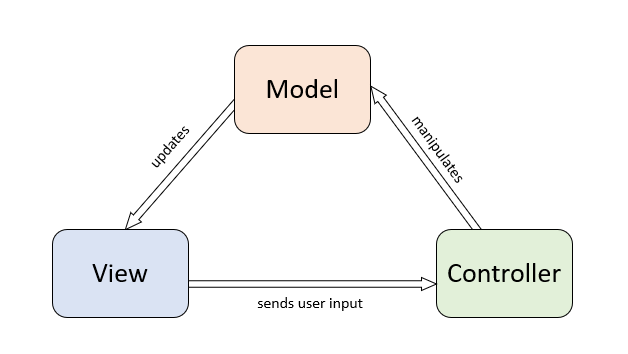
\includegraphics[width=15cm,height=7.5cm,keepaspectratio]{2GrundlagenX/Bilder/MVCArchitecture.png}
    \caption{MVC Architektur Diagramm \cite{mvcbild.2020}}
    \label{pic:mvcdiagram}
\end{figure} 
\\
Im Falle dieser Abbildung wurde das Strukturmuster \ac{MVC} ausgewählt, welches die zu sehenden Komponenten in drei in sich 
geschlossene und unabhängige Fragmente unterteilt die miteinander interagieren. 
\\ 
\linebreak
Neben der Strukturierung von Systemen und Applikationen kann die Modellierung einer Softwarearchitektur auch dabei helfen eine Architektur genauer 
zu beschreiben und zu dokumentieren. Ebenso können Diagramme auch das Management sowie die Planung beeinflussen und verstärken. Die Modellierung 
der Softwarearchitektur stellt somit keinen Selbstzweck dar, sondern bietet einen Mehrwert indem es zur Verständigung, Dokumentation und 
Kommunikation zwischen Entwicklern und Kunden zusätzlich beiträgt. 
\\ 
Durch die Modellierung der Architektur kann frühzeitig eine sinnvolle Evaluierung und Bewertung des Entwurfs durchgeführt werden. Mit diesen 
entstehenden Bewertungen können folgende Schritte besser geplant und umgesetzt werden. 
\\ 
\linebreak
Eine weitere Variante, bzw. Ausprägung der Software-Architektur ist die Modulare Software Architektur (siehe Abschnitt \ref{chap:Modulare Software Architektur}).
Viele Softwarearchitekturen lehnen sich an das Prinzip der Modularen Architektur an und nehmen diese als Grundlage.
\subsection{Modulare Software Architektur}
\label{chap:Modulare Software Architektur}
Der Begriff der Modularität beschreibt den Hauptteil der Architektur. Modularität bezeichnet die Aufteilung eines großen Ganzen in 
mehrere kleinere Teile, die als Module, Komponenten oder Bausteine beschrieben werden. Verschiedene Teile können bei geeigneter Funktion 
und Kompatibilität zusammengeführt werden oder über entsprechend definierte Schnittstellen interagieren. 
\\ 
Unter der allgemeinen modularen Software-Architektur, bzw. Programmierung, versteht man ein Programmierparadigma. Dabei sollte die Software aus 
systematisch und logisch aufgeteilten Teilblöcke bestehen, diese werden Module oder Bausteine genannt. Der Aufbau der modularen Software kann 
praktisch in allen imperativen Programmiersprachen \footnote{Programmierparadigma, das aus einer Folge von Anweisungen besteht.} 
Anwendung finden. Durch Modularität soll die Software bessere Kontrollierbarkeit, Übersichtlichkeit und Testbarkeit innerhalb großer 
Softwareprojekte gewährleisten. So sind die einzelnen Bausteine an sich unabhängig und für sich selbst zuständig, trotz dessen können 
diese mit weiteren Bausteinen kombiniert und verschachtelt werden. 
\\ 
In der Entwicklung sind die einzelnen Module eigenständig und separat zu planen, programmieren und testen. Dadurch ist der Rahmen des 
einzelnen überschaubar und leicht zu praktizieren. Nach erfolgreicher Testung der Module können die Einzelteile als eine Anwendung 
zusammengeführt werden, indem die einzelnen Module logisch über Schnittstellen verknüpft werden. Erst nach diesem Schritt ist die 
entstehende Applikation vollständig einsatzbereit.
\\ 
Die modulare Programmierung gilt als Erweiterung des prozeduralen Ansatzes, dabei sind die Module in kleineren Ansätzen auf die Klassen 
der objektorientierten Programmierung zurückzuführen. \cite{modularesoftware.2018s}
\\
Um eine Software-Architektur übersichtlich und strukturiert umzusetzen, gibt es demzufolge Entwurfsmuster, engl. Patterns, die zusätzlich für 
Ordnung innerhalb der Architektur sorgen. Ein für die Ausarbeitung relevantes Muster ist das MVVM-Pattern. (siehe \ref{chap:MVVM})

\subsection{MVVM}
\label{chap:MVVM}
Das Model-View-ViewModel-Pattern ist, wie bereits erwähnt, ein Architekturmuster das den Entwicklern als Vorlage dient, um ordnungsgemäße, 
standardisierte und strukturierte grafische Oberflächen und das dahinterstehende logische System zu entwickeln. Es wird besonders für 
interaktive Systeme eingesetzt. Das MVVM-Muster wird allgemein als Weiterentwicklung des bekannten MVC-Patterns (der Abbildung \ref{pic:mvcdiagram} zu entnehmen) angesehen. 
\\
Grundlegend ist das Model-View-Controller-Muster, MVC, für die klare Abgrenzung zwischen Daten, deren Darstellung und Präsentation und den 
Nutzerinteraktionen für die graphischen Benutzeroberflächen gedacht. 
\\ 
\linebreak
Demnach ist auch das Model-View-ViewModel-Muster daran angelehnt, die Benutzeroberfläche von deren Logik zu trennen. Durch diese Trennung 
ist eine erhöhte Wartbarkeit und Testbarkeit gewährleistet. Die ermöglichte parallele Arbeitsweise von UI-Designern und Entwicklern 
unterstützt deren Arbeitsfluss und beschleunigt den Entwicklungsprozess. \cite{mvvmentwickler.2010s} 
\\ 
\linebreak
Die Logik der Anwendung wird in den ViewModel-Klassen (\ref{sec:ViewModel}) dargestellt und dienen als Kommunikationsschnittstelle zwischen 
dem Model, dem Datenhalter, und der View, der Datenrepräsentation. Durch die Unabhängigkeit der einzelnen Module kann ein Unit Test vereinfacht 
durchgeführt werden, mitunter ein großer Vorteil des Patterns. 
\\ 
Die Ebenen, die das MVVM-Pattern enthält, werden in Abbildung (\ref{pic:mvvmdiagram}) grafisch aufgeführt.
\begin{figure}[hbt!]
    \centering
    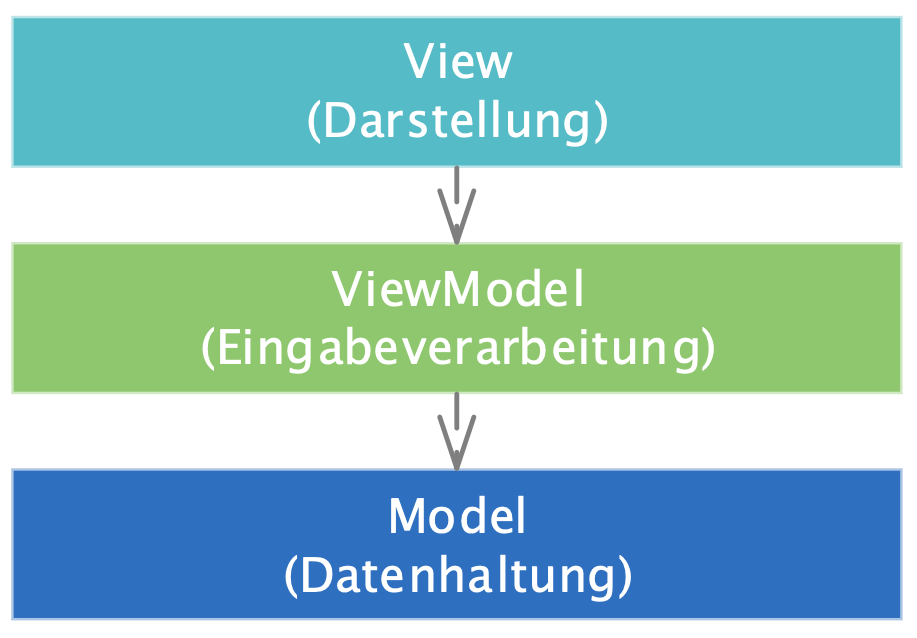
\includegraphics[width=15cm,height=7.5cm,keepaspectratio]{2GrundlagenX/Bilder/mvvmDiagramm.png}
    \caption{MVVM Architektur Diagramm \cite{mvvmDiagramm.2015n}}
    \label{pic:mvvmdiagram}
\end{figure} 
\\
Die View-Ebene stellt die Informationen der Benutzeroberfläche dar, fängt die Benutzereingaben ab 
und gibt diese über Datenbindungen dann an das darunterliegende ViewModel weiter. Die View-Klasse enthält lediglich die Komponenten die 
die Oberfläche optisch aus machen und die dazugehörigen Datenbindungsschnittstellen, um die Informationen übergeben zu können.
Ebenso werden über diese Schnittstelle Informationen geladen, um diese auf der Oberfläche repräsentieren zu können. 
Diese Vorgehensweise erleichtert das Austauschen der View ohne den Code generell zu ändern. 
\\ 
\linebreak 
Die ViewModel, bereits in Kapitel (\ref{sec:ViewModel}) beschrieben, ist dafür zuständig die Daten zwischen der persistierten Speicherung 
und der Repräsentation zu transferieren. Es stellt das Model für die View dar und gibt das eigentliche Model nach außen.
\\ 
\linebreak 
Die unterste Ebene, das Model, bzw. die Datenhaltung, stellt die Abbildung der Daten dar und giltet nicht  als reine Abbildung der Datenquelle. 
Diese Daten werden für die visuelle Anwendung auf der View-Ebene benötigt und durch die ViewModel-Ebene bereitgestellt. Darüberhinaus können die 
Daten von dem Nutzer über die View manipuliert und an das Model zurückgegeben werden. Durch diese Möglichkeiten ist vorausgesetzte, dass das Model 
folgende Funktionalitäten bereitstellen sollte \cite{mvvmAufbau.2016}:
\begin{itemize}
    \item Validierung der Daten
    \item  Benachrichtigung bei Eigenschafts-Änderungen
    \item Verarbeitung von Business-Rules
\end{itemize} 
Sozusagen dient das Model als Schnittstelle zwischen der anhängenden Datenbank und dem ViewModel, welches die Daten hält. 
Dazu kommt, dass das Model festlegt wie die Objekte aufgebaut sind, d.h. dort wird festgelegt welchen Informationen das Objekt beinhaltet. 
\\ 
\linebreak
Die nachfolgende Abbildung (\ref{pic:infoflussmvvm}) veranschaulicht den Informationsfluss des MVVM-Patterns in einzelnen Schritten.
\begin{figure}[hbt!]
    \centering
    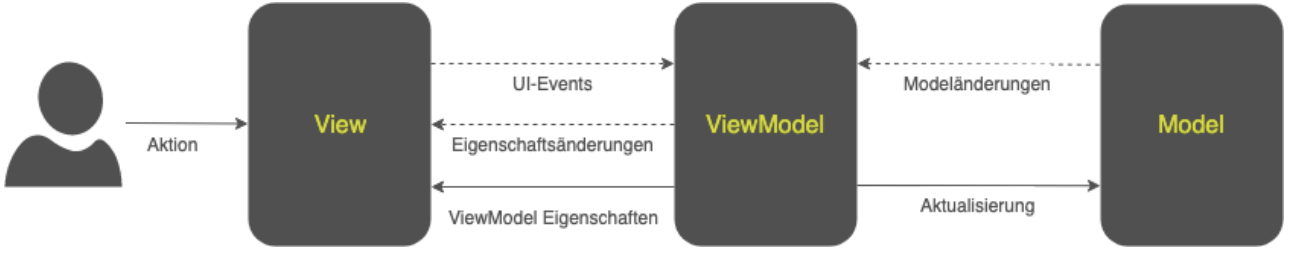
\includegraphics[width=15cm,height=7.5cm,keepaspectratio]{2GrundlagenX/Bilder/infoflussMVVM.png}
    \caption{MVVM Informationsfluss \cite{androidmvvm.2019a}}
    \label{pic:infoflussmvvm}
\end{figure} 
\\ 
\linebreak
Basierend auf der Grundlage des Model-View-ViewModel-Patterns wurde die für das Projekt anvisierte Architektur, Android Architecture Components (\ref{chap:AAC}), 
entwickelt.  
\subsection{Android Architecture Components}
\label{chap:AAC}
Die Android Architecture Components bestehen aus einer Sammlung von Tools und Bibliotheken, engl. Libraries, die entwickelt wurden, um die 
Konstruktion von testbaren und stabilen Android-Apps zu vereinfachen. Mit der Einführung von Android Jetpack (\ref{sec:androidjetpack}) wurden 
viele Komponenten, z.B. Bibliotheken und Frameworks, für die Entwicklung von Apps vereint. In den vielen Bibliotheken, die von Android Jetpack 
zur Verfügung gestellt werden, befinden sich auch die sogenannten \textit{Architecture components}. Diese \textit{Components} unterstützen und 
fördern die Umsetzung der \textit{MVVM} Pattern basierten Architektur (\ref{chap:MVVM}). Die zuvor genannten Bibliotheken ViewModel, LiveData und Room 
sind maßgeblich für die Gestaltung des angestrebten Musters Model-View-ViewModel. 
\\ 
Google selbst empfiehlt im Rahmen der veröffentlichten \textit{„Guide to app architecture“} Dokumentation die Verwendung der \textit{Architecture components}, um 
eine stabile und performante Applikation zu designen, da diese auf bewährten Prinzipien, unter anderem das \textit{seperation of concers} Prinzip, basieren.
\\ 
\linebreak
Folgender Abschnitt befasst sich im einzelnen mit den Komponenten, die für die \textit{Android architecture} essentiell sind:
\begin{figure}[hbt!]
    \centering
    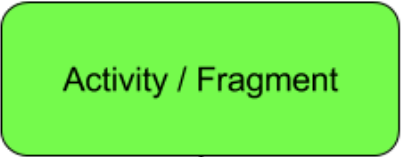
\includegraphics[width=7.5cm,height=5cm,keepaspectratio]{2GrundlagenX/Bilder/activityComp.png}
    \caption{Android Grundkomponente \cite{aac.2020j}}
    \label{pic:activity}
\end{figure}
\\
Grundsätzlich sind Activities und Fragments nicht Teil der eigentlichen \textit{„Architecture Components“}, sondern sind lediglich Grundkomponenten 
der Android App Entwicklung die die Benutzeroberfläche und die dazu korrespondierenden Layout-Dateien verwaltet. 
\begin{figure}[hbt!]
    \centering
    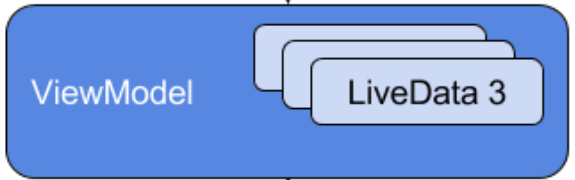
\includegraphics[width=7.5cm,height=5cm,keepaspectratio]{2GrundlagenX/Bilder/viewModelComp.png}
    \caption{ViewModel Komponente \cite{aac.2020j}}
    \label{pic:vmComp}
\end{figure} 
\\ 
Das ViewModel (siehe Abschnitt \ref{sec:ViewModel}) verwaltet die relevanten Daten der UI. Diese Komponente hat einen unabhängigen Lebenszyklus 
dem Activity-Objekt gegenüber. Somit sind Daten bei unvorhergesehenen Unterbrechungen oder Fehlern der UI nicht betroffen und können bei 
erneutem Aufbau der Oberfläche ohne Probleme nachgeladen werden. Die im ViewModel enthaltenen LiveData Objekte (\ref{sec:LiveData}) sind 
beobachtbare Daten-Container die eine Activity ohne expliziten Aufruf über Datenänderungen informiert. Durch diese Methode wird der 
Lebenszyklus der aktiven Komponente respektiert und berücksichtigt. 
\begin{figure}[hbt!]
    \centering
    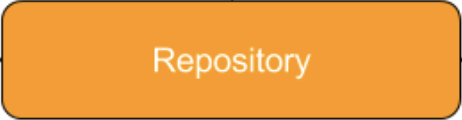
\includegraphics[width=7.5cm,height=5cm,keepaspectratio]{2GrundlagenX/Bilder/repoComp.png}
    \caption{Repository Komponente \cite{aac.2020j}}
    \label{pic:repoComp}
\end{figure} 
\\ 
Mit dem Repository wird ein „best practice“ Fall umgesetzt, der eigentlich kein Bestandteil der Android Jetpack Library ist. Diese Komponente 
ist dafür zuständig das ViewModel von der eigentlichen Datenquelle zu trennen, um Informationen aus verschiedenen Quellen beziehen und 
synchronisieren zu können. Das Repository dient als Schnittstelle zu mehreren Datenbeziehungspunkten und verwaltet ein Verzeichnis zur 
Speicherung und Beschreibung von Objekten und Informationen. Zudem kapselt das Repositorium die Logik für das Persistieren und Erzeugen von 
Entitäten und Aggregaten von der Ansicht. 
\begin{figure}[hbt!]
    \centering
    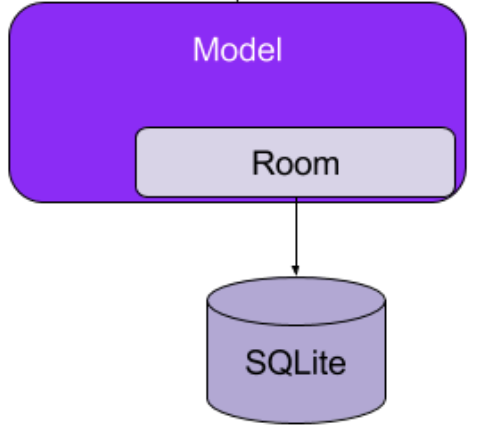
\includegraphics[width=7.5cm,height=5cm,keepaspectratio]{2GrundlagenX/Bilder/roomComp.png}
    \caption{Model / Room Komponente \cite{aac.2020j}}
    \label{pic:roomComp}
\end{figure} 
\\ 
Die \textit{Persistence Library} Room (\ref{sec:Room}) ist ein Datenbank \textit{layer} auf der eigentlichen SQLite Datenbank. Zugriffe auf 
die Datenbank werden durch Room gekapselt und vereinfacht, indem viel mit Annotationen, z.B. \textit{\@Entity, \@Dao}, gearbeitet wird. Der 
Abbildung \ref{pic:roomComp} ist demnach zu entnehmen, dass die Bibliothek Room einen Großteil der Funktionen eines Models abdeckt und so 
die Model-Komponente repräsentiert. Anschließend auf das Datenbank layer ist die eigentliche Persistenzschicht, die SQLite Datenbank.
\\ 
\linebreak 
In einem fortlaufenden Architektur-Diagramm sind die Komponenten wie folgt angeordnet, um die Abhängigkeiten zwischen den einzelnen Teilen 
zu verdeutlichen. 
\begin{figure}[hbt!]
    \centering
    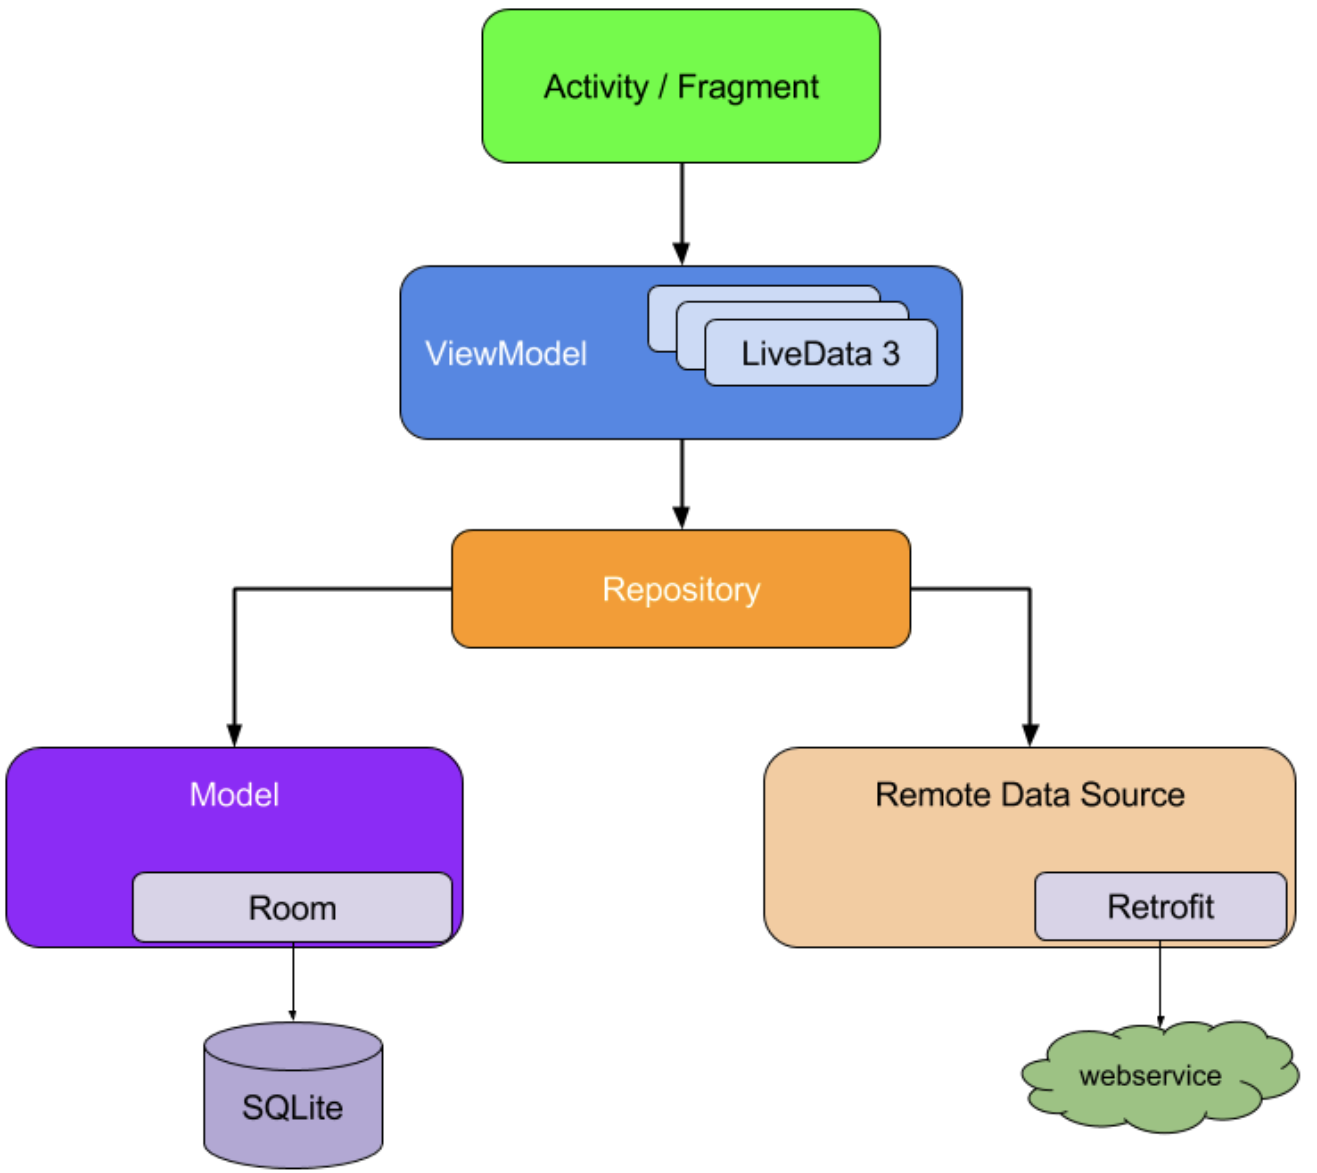
\includegraphics[width=15cm,height=10cm,keepaspectratio]{2GrundlagenX/Bilder/aac.png}
    \caption{Android Architecture Components Diagram\cite{aac.2020j}}
    \label{pic:aacDia}
\end{figure} 
\\ 
In der Abbildung \ref{pic:aacDia} wird deutlich, welches Modul welche Abhängigkeiten besitz, bzw. zu welchen oder von welchen Modulen 
Informationen bezogen werden können. Einzelne Komponenten können ihren Vor- oder Nachgänger niemals umgehen und sind so einer festen 
Hierarchie eingeordnet. Die Abbildung zeigt auch eine beispielhafte Ausführung mehrerer Datenbezugsquellen.
\\ 
Bei genauer Betrachtung des Diagramms sind alle Komponenten wiederzufinden, die ebenso in dem MVVM-Muster gegeben 
sind und das Muster prägen. Durch die vielen Komponenten und Schnittstellen ist modularität gegeben und trägt dazu bei, dass weiter Module 
angehängt oder ausgetauscht werden können. 

\section{Datenmodellierung}
\label{chap:Datenmodellierung}
Datenmodellierung ist ein Verfahren zur formalen Abbildung von Objekten deren Attribute und Beziehungen in einem definierten Kontext. Die 
Modellierung ist zielführend, um einen Überblick der Datensicht des Systems oder der Applikation zu erhalten. Hauptaufgabe ist die eindeutige 
Definition von Objekten und deren Spezifikationen und Ausprägungen. Ebenso hilft die Datenmodellierung bei der visuellen Darstellung von 
Informationen und bei der Einhaltung von Voraussetzungen und Richtlinien.
\\ 
Die aus der Modellierung entstehenden Datenmodelle stellen die Objekte und Beziehungen untereinander dar und repräsentieren die zu 
persistierende Struktur der Objekte. Datenmodelle sind ein wichtiger Bestandteil einer Software und haben meist eine längere Lebensdauer als 
die Software an sich, da Änderungen an den Modellen meist viele Risiken mit sich bringen, überwiegend Datenverlust.
\\ 
\linebreak
Durch die Übersichtlichkeit der Datenmodelle können Standardwerte, Semantik, Sicherheit und die Datenqualität gleichzeitig sichergestellt 
werden. Die Konsistenz von Namenskonventionen wird durch die Überschaubarkeit auch einfacher überprüfbar. 
\\ 
\linebreak
In der Softwareentwicklung wird die Datenmodellierung als wesentliche Teilaufgabe gesehen, um ein System aufzubauen. Innerhalb des 
Datendesigns gibt es drei bedeutsame Varianten die aufeinander aufbauen:
\begin{itemize}
    \item Konzeptionelles Datenbankschema: Betrachtung eines für die Applikation wichtigen Szenarios der realen Welt unter Berücksichtigung 
    aller relevanten Objekte, Eigenschaften und Beziehungen zwischen ihnen. Diese Informationen werden aus dem Kontext heraus analysiert 
    und grafisch als auch textuell dargestellt. Die Darstellung basiert auf einem \ac{ERM}, das die Objekt (Entities) mit ihren jeweiligen 
    Eigenschaften (Attributes) und die Beziehungen (Relationships) darstellt. Das sogenannte Semantische Datenmodell.
    \item Logisches Datenbankschema: Hierbei wird das konzeptionelle Datenbankschema um datentechnische Angaben, z.B. Feldtypen /-formate 
    und Identifikationseigenschaften (Primary Keys), erweitert. Das logische Datenbankschemata unterliegt den Regeln der von dem \ac{DBMS}
    gegebenen Struktur, z.B. dem relationalen Datenmodell, das alle Daten und Objekte in Tabellen ablegt. Auch Relationales oder 
    objektorientiertes Datenmodell genannt. \cite{datenmodellierung.2019d}
    \item Physisches Datenbankschema: Dabei werden die Datensätze auf den physischen Komponenten organisiert und verwaltet. Eine Festlegung 
    der Zugriffsoperationen finden in dieser Phase statt. Zugriffsoperationen sind Einfügen, Löschen, Aktualisieren und Suchen von Objekten 
    und Informationen. Zudem wird hierbei versucht die Performance und effiziente Bearbeitung von Datenbankzugriffen durch Modellierung hochzuhalten.
\end{itemize}  
Die drei oben aufgeführten Phasen sind Bestandteile der Methodik des Datenbankdesigns, der sogenannten \textit{„top down-Methodik“}. 
Wobei die erste Phase die allgemeine Anforderungsanalyse, die in obiger Auflistung nicht aufgeführt ist, beinhaltet. Bei dieser Phase finden 
grundlegende Anforderungsprozesse statt, zum einen die Informationsstrukturanforderungen und zum anderen die Datenverarbeitungsanforderungen. 